%% Change "letterpaper" in the following line to "a4paper" if you must.

\documentclass[10pt,a4paper]{article}
\usepackage{cogsci}
\usepackage{pslatex}
\usepackage{apacite}


%\usepackage{geometry}
\usepackage{natbib}
\bibpunct[:]{(}{)}{,}{a}{}{;}

\usepackage{amsmath}
\usepackage{amsfonts}
\usepackage{amsthm}
\usepackage{amssymb}
\usepackage{mathrsfs}
\usepackage{nicefrac}
%\usepackage{stmaryrd}
%\usepackage{multicol}
\usepackage{graphicx}
\usepackage{caption}
\usepackage{subcaption}
\usepackage{color}
\usepackage{booktabs}

\usepackage{blkarray}
\usepackage{xspace}


\definecolor{Red}{RGB}{178,34,34}
\newcommand{\mf}[1]{\textcolor{Red}{[MF: #1]}} 
\newcommand{\tb}[1]{\textcolor[rgb]{.8,.33,.0}{[TB: #1]}}% prints in orange
\newcommand{\citeposs}[2][]{\citeauthor{#2}'s (\citeyear[#1]{#2})}
\newcommand{\tuple}[1]{\ensuremath{\left\langle #1 \right\rangle}} 


%%% MF's commands
\newcommand{\set}[1]{\left\{#1\right\}}
\newcommand{\card}[1]{\left \lvert \, #1 \, \right\rvert}
\newcommand{\abs}[1]{\lvert #1 \rvert}
\newcommand{\States}{\ensuremath{S}\xspace}		% Set of States
\newcommand{\state}{\ensuremath{s}\xspace}		% single states
\newcommand{\mystate}[1]{\ensuremath{\state_{\text{#1}}}\xspace} %meaningful states
\newcommand{\Messgs}{\ensuremath{M}\xspace}		% Set of Messages
\newcommand{\messg}{\ensuremath{m}\xspace}		% single messages
\newcommand{\mymessg}[1]{\ensuremath{\messg_{\text{#1}}}\xspace} %meaningful messages
\newcommand{\ssome}{\mystate{\ensuremath{\exists\neg\forall}}}
\newcommand{\sall}{\mystate{\ensuremath{\forall}}}
\newcommand{\msome}{\mymessg{some}}
\newcommand{\mall}{\mymessg{all}}
\newcommand{\asome}{\myact{\ensuremath{\exists\neg\forall}}}
\newcommand{\aall}{\myact{\ensuremath{\forall}}}
\newcommand{\type}[1]{\ensuremath{\tau_{#1}}}
\newcommand{\postparameter}{\ensuremath{\gamma}}
\definecolor{mygray}{cmyk}{0.35,0.35,0.35,0.35}
\newcommand{\mygray}[1]{{\textcolor{mygray}{#1}}}


%\interfootnotelinepenalty=10000 %force footnote on same page


%\citeA{bibkeyword} cites only year

\title{Effects of transmission perturbation in the cultural evolution of language}
 
\author{{\large \bf Thomas Brochhagen (t.s.brochhagen@uva.nl)}\\
  Institute for Logic, Language \& Computation, University of Amsterdam
  \AND {\large \bf Michael Franke (mchfranke@gmail.com)} \\
  Department of Linguistics, University of T\"{u}bingen}


\begin{document}
\maketitle

\begin{abstract}
  Two factors seem to play a major role in the cultural evolution of language. On the one hand,
  there is functional pressure towards efficient transfer of information. On the other hand,
  languages have to be learned repeatedly and will therefore show traces of systematic
  stochastic disturbances of the transmission of linguistic knowledge. While a lot of attention
  has been paid to the effects of cognitive learning biases on the transmission of language,
  there is reason to expect that the class of possibly relevant transmission perturbations is
  much larger. This paper therefore explores some potential effects of transmission noise due
  to errors in the observation of states of the world. We look at three case studies on (i)
  vagueness, (ii) meaning deflation, and (iii) underspecified lexical meaning. These case
  studies suggest that transmission perturbations other than learning biases might help explain
  attested patterns in the cultural evolution of language and that perturbations due to
  perceptual noise may even produce effects very similar to learning biases.

\textbf{Keywords:} 
cognitive biases; iterated learning; language evolution  
\end{abstract}


\section{Introduction}

Language is shaped by its use and transmission across generations. Linguistic properties are
therefore not necessarily solely due to functional pressure, such as the selection of more
communicatively efficient behavior. They may also be effected by a pressure for
learnability. In the extreme, an unlearnable language will not make it to the next
generation. The effects that (iterated) learning has on language are often seen as stemming
from a combination of general learning mechanisms and inductive cognitive biases
(e.g. \citealt{griffiths+kalish:2007,kirby+etal:2014,tamariz+kirby:2016}). Proposals of biases
that shape language acquisition abound, e.g.; mutual exclusivity
\citep{merriman+bowman:1989,clark:2009}, simplicity \citep{kirby+etal:2015}, regularization
\citep{hudson+etal:2005}, and generalization \citep{smith:2011}. But forces other than learning biases may also systematically perturb the transmission of
linguistic knowledge and thereby contribute to the shaping of language by
cultural evolution \citep[cf.][]{perfors+navarro:2014}.  In the following we focus on one particular source of transmission noise:
agents' imperfect perception of the world. Our overall goal is to give a
formalism with which to study the possible effects of such perturbations and to apply it to
three case studies on (i) vagueness, (ii) meaning deflation, and (iii) underspecified lexical
meaning.

\section{Iterated Bayesian learning}

We model the transmission of linguistic knowledge as a process of iterated learning \citep{kirby+etal:2014, tamariz+kirby:2016}.
More specifically, we focus on
iterated Bayesian learning, in which a language learner must infer unobservables, such as the
lexical meaning of a word, from the observable behavior of a single teacher, who is a
proficient language user \citep[e.g.][]{griffiths+kalish:2007,kirby+etal:2007}. Concretely, the
learner observes instances $\tuple{s,m}$ of overt language use in context, where $s$ is a world state
and $m$ is the message that the teacher used in state $s$. The learner's task is to infer which
latent type \type{} (e.g., which set of lexical meanings or which grammar) may have produced a
sequence of such observations. To do so, the learner considers the posterior probability of \type{} given a data sequence $d$ of $\tuple{s, m}$ pairs:
\begin{align*}
  P(\type{} \mid d) \propto P(\type{}) \ P(d \mid \type{})\,,
\end{align*}
where $P(\type{})$ is the learner's prior for type \type{} and
$P(d \mid \type{}) = \prod_{\tuple{s,m} \in d} P(m \mid s, \type{})$ is the likelihood of type \type{}
producing the observed data $d$, with $P(m \mid s, \type{})$ the probability that a type \type{} produces
message $m$ when in world state $s$. It is usually assumed that learners exposed to $d$ adopt
type \type{} with probability $F(\type{} \mid d) \propto P(\type{} \mid d)^\postparameter$, where $\postparameter \ge 1$ regulates
whether learners probability match ($\postparameter = 1$) or tend towards choosing a maximum of the
posterior distribution ($\postparameter > 1$). If the set $D_k$ of data a learner may be exposed to is the
set of all sequences with $k$ pairs $\tuple{s,m}$, the probability that a learner acquires type
\type{i} when learning from a teacher of type \type{j} is:
\begin{align*}
  P(\type{j} \rightarrow \type{i}) &\propto \sum_{d \in D_k} P(d \mid \type{j}) F(\type{i} \mid d)\,.
\end{align*}
If a population is a distribution over types, then iterated Bayesian learning predicts the most
likely path of change in the population due to learning from finite observations.

The prior $P(\type{})$ can be understood as encoding learning biases. For example, learners may have
an a priori preference for simpler languages over ones with a more complex grammar, or over
ones with larger or more marked lexical or phonemic inventories
(cf. \citealt{chater+vitanyi:2003, kirby+etal:2015}). Crucially, even weak biases
can magnify and have striking effects on an evolving linguistic system, especially if learning
is fueled by only limited input (small $k$). Experimental and mathematical explorations of
iterated learning have consequently suggested that the linguistic structure evinced by the outcome of this process
reflects learners' inductive biases \citep{kirby+etal:2007,kirby+etal:2014}.

%The role of such biases can be viewed as that of
%introducing systematic perturbations in the transmission of linguistic knowledge, guiding
%learners to the convergence on particular evolutionary outcomes.

\section{Iterated Bayesian learning with state-noise}

Other stochastic factors beyond learning biases in $P(\type{})$ can influence the adoption of a
linguistic type $\type{}$ based on the observation of $\tuple{s,m}$ sequences. One further potential source
of ``transmission noise'' are regular stochastic errors in the perception of world states (see
Figure~\ref{fig:cartoon}).
%
\begin{figure}[t]
  \centering
  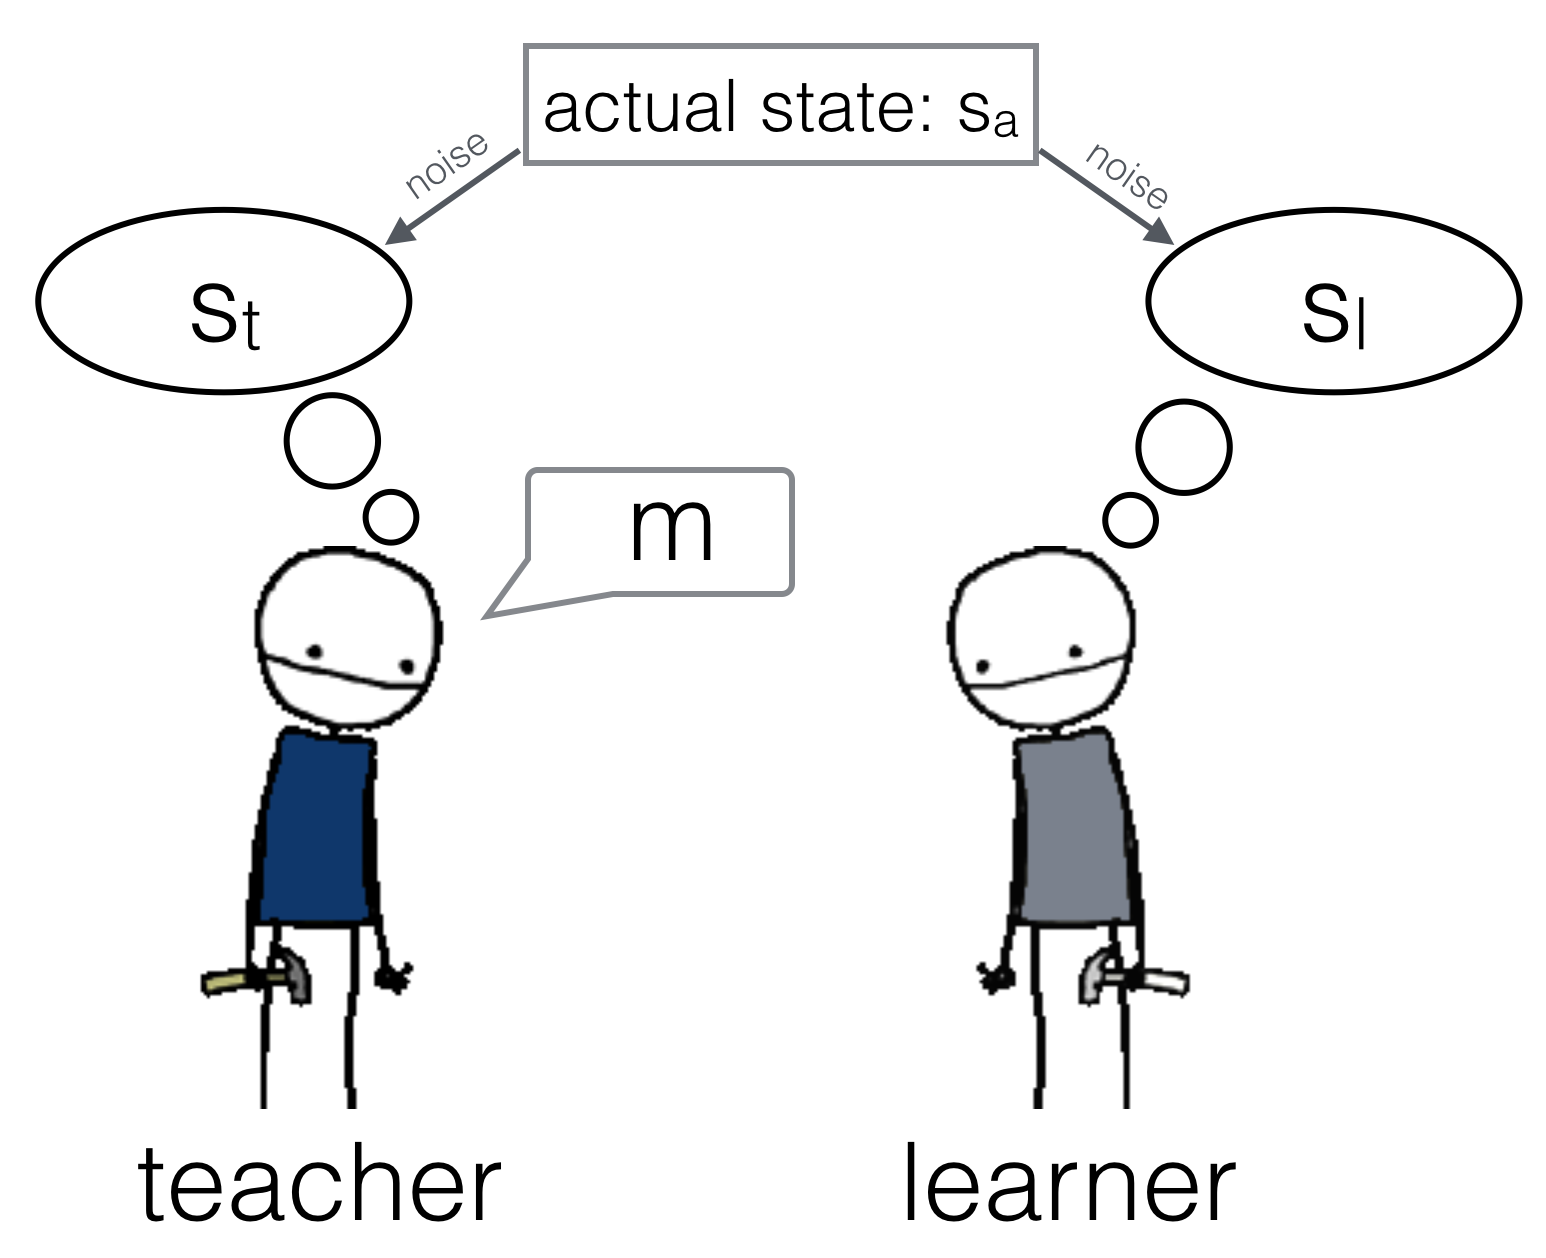
\includegraphics[width = 0.75\linewidth]{pics/cartoon_picture.png}
  \caption{State-noise during observation of language use.}
  \label{fig:cartoon}
\end{figure}
% 
Imperfect perception may lead teachers to produce utterances that deviate from
their production behavior had they witnessed the state correctly. Similarly, learners may
mistake utterances as applying to different states than the ones witnessed by the teacher who
produced them. For instance, when learning the meaning of a vague adjective such as {\em tall}
from utterances like ``Jean is tall'', agents may have diverging representations of how tall
Jean actually is, even if she is in a shared perceptual environment. The main idea to be
explored here is that regularities in misperceptions of states may have striking and possibly
explanatory effects on language evolution.

We denote the probability that the teacher (learner) observes state $s_t$ ($s_l$) when the actual state is $s_a$ as $P_N(s_t \mid s_a)$ ($P_N(s_l \mid s_a)$). The probability that $s_a$ is the actual state when the learner observes $s_l$ is therefore:
\begin{align*}
  P_N(s_a \mid s_l) \propto P(s_a) \ P_N(s_l \mid s_a)\,.
\end{align*}
Assuming a finite state space for convenience, the probability that the teacher observes $s_t$
when the learner observes $s_l$ is:
\begin{align*}
  P_N(s_t \mid s_l) = \sum_{s_a} P_N(s_a \mid s_l) \ P_N(s_t \mid s_a)\,.
\end{align*}
The probability that a teacher of type \type{} produces data that is perceived by the learner as a
sequence $d_l$ of $\tuple{s_l, m}$ pairs is:
\begin{align*}
  P_N(d_l \mid \type{}) = \prod_{\tuple{s_l,m} \in d_l} \sum_{s_t} P_N(s_t \mid s_l) \ P(m \mid s_t, \type{})\,.
\end{align*}
It is natural to assume that learners, even if they (in tendency) perform rational Bayesian
inference of the likely teacher type $\type{}$ based on observation $\tuple{s_l,m}$, do not also
reason about state-noise perturbations. In contrast to, e.g., noisy-channel models that have agents reason over potential
message corruption caused by noise \citep[e.g.][]{bergen+goodman:2015}, our learners are not proficient language users that could leverage knowledge about the world and its linguistic codification  to infer likely state misperception.\footnote{To do so, agents would have to infer or come equipped with knowledge about $P_N(\cdot|s_a)$, which could itself be
subject to updates. We stick to the simpler case of ignorance about noise here, but as long as the actual state is not always recoverable our general results also hold for agents that reason about noise.} In this case the posterior probability of $\type{}$ given the
learner's perceived data sequence $d_l$ is as before:
$P(\type{} \mid d_l) \propto P(\type{}) \ P(d_l \mid \type{})$.  Still, state-noise affects the probability
$P_N(\type{j} \rightarrow \type{i})$ that the learner adopts $\type{i}$ given a teacher of type $\type{j}$, because
it influences the probability of observing a sequence $d_l$ (with $F(\type{i} \mid d)$ as before):
\begin{flalign*}
  P_N(\type{j} \rightarrow \type{i}) \propto \sum_{d \in D_k} P_N(d_l \mid \type{j}) F(\type{i} \mid d)\,.
\end{flalign*}
% Noise free iterated Bayesian learning is obtained as a special case when the perceived state is
% always the actual state.

% Finally, we need to specify what the transmission matrix $Q$ operates over. This could be a distribution over types that an agent in the learning chain entertains at a given time, but also as a population of types following standard practice in evolutionary game theory (for discussion on the relationship of single chain learning and population dynamics see e.g. \citealt[\S 7]{griffiths+kalish:2007}). Here, we adopt the latter view, and consequently take this component to be a population vector $x$, where $x_i$ is the proportion of type $t_i$ in $x$. The full dynamics are captured by the discrete mutator dynamics $\hat{x}_j = \sum_i Q_{ij} x_j$ (for an overview see \citealt{hofbauer+sigmund:2003}).

In sum, it may be that learner and/or teacher do not perceive the actual state as what
it is. If they are not aware of this, they produce/learn as if what they observed was the
actual state. In particular, the learner does not reason about noise when she tries to infer
the teacher's type. She takes what she observes as the actual state that the teacher has seen
as well, and infers which linguistic type (e.g. which set of lexical meanings or grammar) would have
most likely generated the message to this state. This
can lead to biases of inferring the ``wrong'' teacher type if noise makes some types err in a
way that resembles the noiseless behavior of other types. That is, such environmental factors
can, in principle, induce transmission perturbations that look as if there was a cognitive bias
in favor of a particular type, simply because that type better explains the noise.


\section{Case studies}

In what follows we present three case studies that show how iterated learning under noisy
perception can lead to the emergence of linguistic phenomena. The 
studies are ordered from more to less obvious examples in which state-noise may be influential
and explanatory: (i) vagueness, (ii) meaning deflation, and (iii) underspecification in the
lexicon.
% The first study on vagueness shows that, if concerns the emergence of vagueness in a community of language users
% that initially makes sharp linguistic distinctions between states. The second study considers a
% similar setup in which agents start out by using an expression only for a small subset of
% states. Over time, the strict boundary set by the initial language is shown to relax, leading
% to an iterated expansion of the expression's range over the state space. That is, meaning
% deflates as a consequence of transmission perturbations caused by noise. Finally, we analyze a
% subset of \citeposs{brochhagen+etal:2016:CogSci} case study on the lexicalization of a lack of
% upper-bounds in the meaning of weak scalar expressions. As in the preceding cases, we show how
% certain noise patterns can give rise to outcomes predicted by theoretical and empirical
% investigations.
No case study is meant to suggest that state-noise is the definite and only explanation of the
phenomenon in question. Instead, our aim is to elucidate the role that transmission perturbations beyond
inductive biases may play in shaping the cultural evolution of language. We therefore present
minimal settings that isolate potential effects of state-noise in iterated learning.

%Note also that constructing the set of learning data $D$ is computationally intractable for
%large $k$. We therefore approximate $D$ by sampling data from the production behavior of
%types. The values chosen correspond to experimentally determined amounts that minimize the
%effects that insufficient sampling may otherwise introduce. \mf{I would probably skip
%  this. Technical details are backgrounded here anyway, and have to be.}

\subsection{Vagueness}

Many natural language expressions are notoriously vague and pose a challenge to logical
analysis of meaning \citep[e.g.][]{Williamson1994:Vagueness}. Vagueness also challenges models
of language evolution since functional pressure towards maximal information transfer should,
under fairly general conditions, weed out vagueness \citep{Lipman2009:Why-is-Language}. Many
have therefore argued that vagueness is intrinsically useful for communication
\citep[e.g.][]{Deemter2009:Utility-and-Lan,Jaegherde-JaegherRooijvan-Rooij2010:Strategic-Vague,BlumeBoard2013:Intentional-Vag}. Others
hold that vagueness arises naturally due to limits of perception, memory, or information
processing
\citep[e.g.][]{FrankeJager2010:Vagueness-Signa,OConnor2013:The-Evolution-o,LassiterGoodman2015:Adjectival-vagu}. We
follow the latter line of exploration here, showing that vagueness can naturally arise under
imperfect observability of states (see \cite{franke+correia:toappear} for a different
evolutionary dynamic based on the same idea).

\paragraph{Setup.}  We analyze the effects of noisy perception on the transmission of a simple
language with $100$ states, $s \in [0,99]$, and two messages, $m \in \{m_1,m_2\}$. The
probability that agents perceive actual state $s_a$ as perceived $s_t$/$s_l$ is given by a (discretized) normal
distribution, truncated to $[0;99]$, with $s_a$ as mean and standard deviation
$\sigma$. % That is, $P(s_p | s_a) \sim \text{Normal}(s_{a},\sigma,s_{0},s_{99})$ with
% $\sigma$ controlling the degree to which states are confused, and as boundaries $s_{0}$ and
% $s_{99}$.
Linguistic behavior is fixed by a type $\type{} \in [0;99]$ which is the threshold of applicability
of $m_1$: $P(m_1 \mid s,\type{}) = \delta_{s \ge \type{}} = (1 - P(m_2 \mid s,\type{}))$. In words, if a speaker observes a
state that is as large or larger than its type, then message $m_1$ is
used (\emph{tall}), otherwise $m_2$ ({\em small}).

\paragraph{Results.} The effects of a single generational turnover under noisy transmission of a population that initially consisted exclusively of type $\type{} = 50$ is
depicted in Figure \ref{fig:vag}. As learners try to infer this type from observed language use, even small $\sigma$ will lead to
the emergence of vagueness in the sense that there is no longer a crisp and determinate cut-off
point for message use in the population. Instead, \emph{borderline regions} in which $m_1$ and $m_2$
are used almost interchangeably emerge. For larger $\sigma$, larger borderline regions ensue. The size
of such regions further increases over generations with growth inversely related to $\postparameter$
and $k$. As is to be expected, if $k$ is too small to discern even strikingly different types,
then iterated learning under noisy perception leads to heterogeneous populations with (almost)
no state being (almost) exclusively associated with $m_1$ or $m_2$.

\begin{figure}[ht]
\centering
    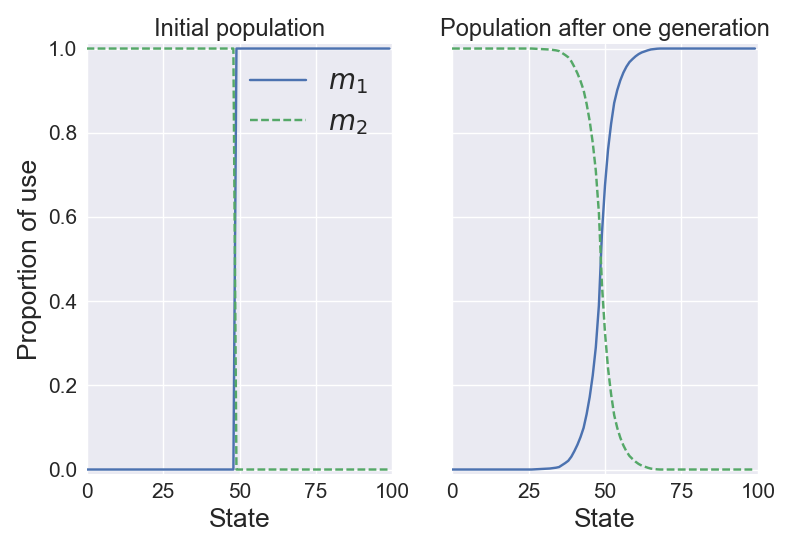
\includegraphics[width=\textwidth,height=6.15cm, keepaspectratio]{../code/plots/vag-side-by-side.png}
\caption{Noisy iterated learning with posterior sampling ($\postparameter=1$), $\sigma = 0.4$, and $k = 20$.}
  \label{fig:vag}
\end{figure}
 
\paragraph{Discussion.}
Transmission perturbations caused by noisy state perception reliably give rise to vague
language use even if the initial population had a perfectly crisp and uniform
convention. Clearly, this is a specific picture of vagueness. As modeled here for simplicity,
each speaker has a fixed and non-vague cut-off point $\type{}$ in her lexicon. Still, the production
behavior of a type-$\type{}$ speaker in actual state $s_a$ is probabilistic and ``vague'', because of
noisy perception:
\begin{align*}
  P_N(m \mid s_a, \type{}) = \sum_{s_p} P(s_p \mid s_a) P(m \mid s_p, \type{})\,.
\end{align*}
An extension towards types as distributions over thresholds is straightforward but the main
point would remain: systematic state-noise perturbs a population towards vagueness. 

Of course, convergence on any particular population state will also depend on the functional
(dis)advantages of particular patterns of language use. Functional pressure may therefore well
be necessary for borderline regions to be kept in check, so to speak. Which factor or
combination thereof plays a more central role for the emergence of vagueness is an empirical
question we do not address here. Instead, we see these results as adding strength to the
argument that one way in which vagueness may arise is as a byproduct of interactions between
agents that may occasionally err in their perception of the environment. If state perception is
systematically noisy and learners are not aware of this, some amount of vagueness may be the
natural result.

\subsection{Deflation}
Meaning deflation is a diachronic process by which a form's once restricted range of
applicability broadens. Perhaps the most prominent example is Jespersen's cycle
\citep{dahl:1979}, the process by which emphatic negation, such as French {\em ne ... pas},
broadens over time and becomes a marker for standard negation. As argued by
\citet{bolinger:1981}, certain word classes are particularly prone to slight and unnoticed
reinterpretation. When retrieving their meaning from contextual cues, learners
may consequently continuously spread their meaning out. For instance, Bolinger discusses how the indefinite
quantifier {\em several} has progressively shifted from meaning {\em a respectable number} to
broader {\em a few} in American English. We follow this line of reasoning and show how state
confusability may lead to meaning deflation. Other formal models of deflationary processes in
language change have rather stressed the role of conflicting interests between interlocutors
\citep{AhernClark2014:Diachronic-Proc} or asymmetries in production frequencies during learning
\citep{Schaden2012:Modelling-the-A,Deo2015:The-Semantic-an}.


\paragraph{Setup.} The setup is the same as that of the previous case study, except that
we now trace the change of a single message $m$, e.g., emphatic negation, without a fixed
antonym being sent whenever $m$ does not apply. This is a crude way of modeling use of
markers of emphasis or high relevance for which no corresponding ``irrelevance marker''
exists. Learners accordingly observe positive examples of use $\tuple{s,m}$ but do not
positively observe situations in which $m$ did not apply to a particular state. This causes
asymmetry in the learning data because some types will reserve their message only for a
small subset of the state space and otherwise remain silent. Learners take the absence of
observations into account but cannot know what it is that they did not observe. We assume that
learners are aware of $k$ so that:\footnote{Knowing $k$ allows learners to compute the
  likelihood of a type not reporting $k -|d_l|$ state observations. A better but more complex
  alternative is to specify a prior over $k$ with learners performing a joint inference on $k$
  and the teacher's type. For simplicity, we opt for the former, albeit admittedly artificial,
  assumption.}
\begin{align*}
  P(\type{} | d_l) & \propto \text{Binom}(\text{successes} =
  k-|d_l|, \text{trials} = k, \\
  & 
  \ \ \ \ \ \text{succ.prob} = \sum_{i=0}^{\type{}-1} P(s = i)) \prod_{s \in d_l} P(m|s,\type{})\,.
\end{align*}
As before, the second factor corresponds to the
likelihood of a type producing the perceived data.  The first is the probability of a type not
reporting $k-|d|$ events for a total of $k$ events. $P \in \Delta(S)$ is assumed to be
uniform. In words, a long sequence of data consisting of mostly silence gives stronger evidence
for the type producing it having a high threshold of applicability even if the few state-message pairs observed may be equally likely to be produced by types with lower thresholds.

\paragraph{Results.} The development of an initially monomorphic population consisting only of
$\type{} = 80$ is shown in Figure \ref{fig:defl}. Even little noise causes a message to gradually be
applied to larger portions of the state space. The speed of meaning deflation is regulated by
$\sigma$, $k$, and to lesser degree $\postparameter$. In general, more state confusion due to higher
$\sigma$, shorter sequences, or less posterior maximization will lead to more learners
inferring lower types than present in the previous generation.

\begin{figure}[ht]
\centering
    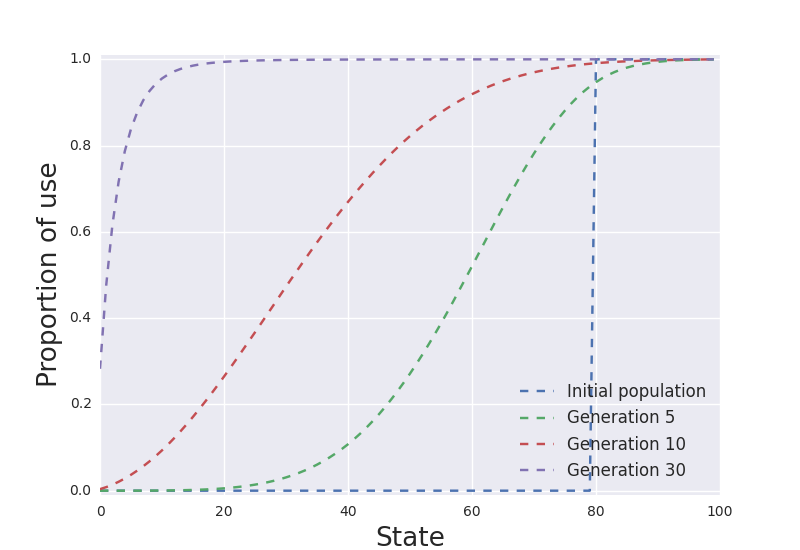
\includegraphics[scale=0.4]{../code/plots/deflation-sigma04.png}
  \caption{Noisy iterated learning with posterior sampling ($\postparameter=1$), $\sigma = 0.4$, and $k = 30$.}
  \label{fig:defl}
\end{figure}

\paragraph{Discussion.} In contrast to the previous case study, we now considered the effects
of noisy perception under asymmetric data generation where overt linguistic evidence is not
always produced, i.e., acquisition in a world in which not every state is equally likely to lead to an observable
utterance. %(coupled with the idealized assumption that learners are aware of the amount of silence ``produced'' by a teacher).

The outcome is similar to that of the previous study. Noisy perception can cause transmission
perturbations that gradually relax formerly strict linguistic conventions. In contrast to the
case of vagueness, if there are no relevant competing forms, e.g., {\em small} vs. {\em tall},
asymmetry in production and noise will iteratively increase the state space that a form carves
out.

\subsection{Scalar expressions}
Scalar expressions have been at the center of many studies on pragmatic inference. Examples
include quantifiers such as {\em some} and {\em most}, adjectives such as {\em cold} and {\em
  big}, and numerals such as {\em four} and {\em ten}. Commonly, their use is taken to
pragmatically convey an upper-bound which is not present in their lexical semantics
\citep{horn:1972,gazdar:1979}. For instance, while ``Bo ate some of the cookies'' is
semantically compatible with a state in which Bo ate all of them, this utterance is often taken to convey 
that Bo ate {\em some but not all}, as otherwise the speaker would have said {\em all}. A
semantically weak meaning is thus pragmatically strengthened by interlocutors' mutual reasoning
about rational language use \citep{grice:1975}. 

Why does such pragmatic strengthening not lead to wide-spread lexicalization of upper-bounded
meanings? To address this question, \citet{brochhagen+etal:2016:CogSci} explore an evolutionary
model that combines functional pressure and iterated learning.  This account assumes a prior
that favors a lack of upper-bounds. Here, we demonstrate that state-noise can mimic the effects
of such a cognitive learning bias.

\paragraph{Setup.} The simplest possible model distinguishes two kinds of lexica and two
behavioral strategies to use them, a pair of which constitutes a type. Both lexica specify the
truth-conditions of two messages in either of two states. Let us mnemonically label them
$\msome$, $\mall$, $\ssome$ and $\sall$, where the former state is one in which natural
language {\em some but not all} holds, and the latter one where {\em all} holds. In lexicon
$L_{\text{bound}}$, which lexicalizes an upper-bound for {\em some}-like expressions, message $\msome$ is only true of $\ssome$ and $\mall$ only of $\sall$. In
the English-like lexicon $L_{\text{lack}}$, message $\mall$ is also only true of $\sall$, but the
meaning of $\msome$ is underspecified and lexically holds in both states.  Speakers follow one of two strategies of language use: literal or pragmatic. 
The former select a random true message, whereas the latter prefer to send the most informative messages from those that are true in
the observed state \citep{grice:1975}. This gives rise to probabilistic speaker behavior
$P(m \mid s,\type{}= \tuple{\text{lexicon},\text{use}})$ which approximates the following choice
probabilities:\footnote{Concretely, results are obtained for probabilistic speaker behavior
  following the definitions of \citet{brochhagen+etal:2016:CogSci}. Nothing essential to our
  main argument and simulation results hinges on these details, so we background them here for
  ease of exposition.}

\begin{centering}
\hspace{2cm} \underline{$L_{\text{bound}}$} \hspace{2.8cm} \underline{$L_{\text{lack}}$} \hspace{1.2cm}\\
\underline{Literal} \hspace{0.6cm}  \bordermatrix{~ & \msome & \mall \cr 
                  \sall & 0 & 1 \cr
                  \ssome & 1 & 0 \cr} \hspace{0.5cm} \bordermatrix{~ & \msome & \mall \cr 
                  \sall & 0.5 & 0.5 \cr
                  \ssome & 1 & 0 \cr}\\[0.25cm]
\underline{Pragmatic} \hspace{0.05cm}  \bordermatrix{~ & \msome & \mall \cr 
                  \sall & 0 & 1 \cr
                  \ssome & 1 & 0 \cr} \hspace{0.45cm} \bordermatrix{~ & \msome & \mall \cr 
                  \sall & 0 & 1 \cr
                  \ssome & 1 & 0 \cr},\\[0.5cm]
\end{centering}

\noindent where $P(m|s,\type{}) = M_{[s,m]}$ with $M$ being type \type{}'s choice matrix.

As pragmatic users of $L_\text{lack}$ are (almost) indistinguishable from types with
$L_\text{bound}$, the emergence of a predominance of $L_\text{lack}$ in a repeatedly learning
population must come from transmission biases. A learning bias in favor of $L_\text{lack}$ in
the learners' priors will select for it \citep{brochhagen+etal:2016:CogSci}, but here we assume
no such cognitive bias. Rather we assume state-noise in the form of parameters $\epsilon$ and
$\delta$. The former is the probability of perceiving actual state $\ssome$ as
$\sall$, $P(\sall | \ssome) = \epsilon$, and $P(\ssome | \sall) = \delta$. For instance, states
may be perceived differently because different numbers of objects must be perceived (e.g.,
quantifiers and numerals) or they may be more or less hard to accurately retrieve from sensory
information (e.g., adjectives).


\paragraph{Results.} To quantify the effects of the dynamics we ran a fine-grained parameter
sweep over $\epsilon$ and $\delta$ with $50$ independent simulations per parameter
configuration. Each simulation started with a random initial population distribution over types
and applied iterated learning with state-noise for $20$ generations, after which no noteworthy change was registered.
Mean proportions of resulting pragmatic users of $L_{\text{lack}}$ under different noise signatures are shown in Figure
\ref{fig:quant}. These results suggest that when $\delta$ is small and $\epsilon$ high, iterated noisy transmission can
lead to populations consisting of almost exclusively English-like lexica with pragmatic
language use. Similar results are obtained for larger $k$ or \postparameter.

\begin{figure}[ht]
\centering
    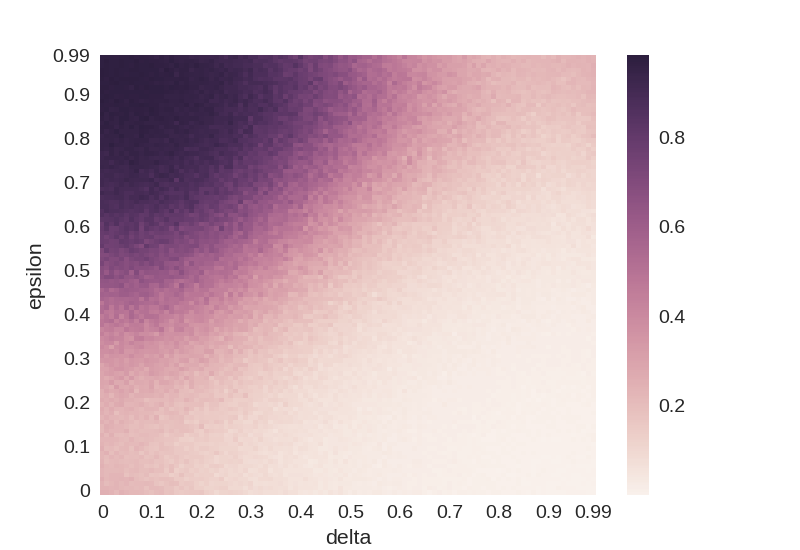
\includegraphics[scale=0.33]{../code/plots/quantifiers-posterior-sampling-k5.png}
  \caption{Mean proportion of pragmatic $L_{\text{lack}}$ users after $20$ generations with posterior sampling ($\postparameter = 1$) and $k = 5$.}
  \label{fig:quant}
\end{figure}


\paragraph{Discussion.} The main goal of this case study was to show that noisy perception may
mimic effects of learning biases. In the case of Brochhagen et al. the assumed bias was one
for simplicity; learners had an a priori preference for not codifying 
upper-bounds lexically, which increased their propensity to infer pragmatic
$L_{\text{lack}}$ over $L_{\text{bound}}$ even if the witnessed data could not tease them
apart. We assumed no such bias but nevertheless arrived at an evolutionary outcome that
is comparable to the one predicted if the bias were present. However, this outcome
strongly depends on the types involved. Whether a type thrives under a particular noise
signature depends on the proportion of types confused with it during transmission. The addition
or extraction of a single type may therefore lead to different results.

At present, it is unclear what role noisy perception should play in the selection of underspecified meaning. These results should therefore be taken as suggestive but not indicative of a relationship between the two. In the case of quantifiers, a possible way to explore this relation may lie in their connection to empirical work on the verification of quantified statements (see \citealt{szymanik:2016} for a recent overview). The idea being that some states are easier to verify, e.g., $\sall$, and therefore less confusable with other states than others, e.g., $\ssome$. 


\section{General discussion}
We proposed a general model of iterated Bayesian learning that integrates systematic noise in agents'
perception of world states, giving rise to stochastic perturbations that may influence and
(potentially, partially) explain language change. We investigated the model's predictions in
three case studies that show that iterated noisy transmission can lead to outcomes akin to
those found in natural language. As stressed before, these results are not meant to suggest
noisy perception to be the sole or main determinant of these phenomena. Instead, our aim was
mainly conceptual and technical in nature.

Beyond technical aspects, we foregrounded two intertwined issues in the cultural evolution of
language. First, the fact that noise signatures may mimic the effects of cognitive biases has
consequences for the interpretation of outcomes of acquisition processes. Care must
therefore be exercised in reading off the influence of possible learning biases from
data obtained ``in the wild'' or the laboratory. Noisy perception can instead be regarded as a neutral
model of cultural evolution as it does not appeal to functional
competition nor differential learnability among types \citep{reali+griffiths:2009}. Second, and more importantly, these results
may be seen as complementing and stressing the pivotal role of systematic transmission
perturbations as explanatory and predictive devices of language change -- independent of the
perturbation's source. They thereby strengthen and widen the scope of research on iterated
learning by bringing attention to forces beyond inductive biases \citep[cf.][]{perfors+navarro:2014}.


\section{Conclusion}
Acquisition is a central force shaping linguistic structure. The consideration of the
(imperfect) means by which such knowledge is transmitted is therefore crucial to our
understanding of the cultural evolution of language. Here, we focused on one factor that may
give rise to systematic stochastic perturbation in learning ---agents' noisy perception of the
world--- and analyzed its effects in three case studies on (i) vagueness, (ii) meaning
deflation, and (iii) underspecified lexical meaning. Our results suggest that the class of
relevant perturbation sources reaches beyond the well-studied effects of inductive learning
biases. In particular, that some linguistic properties, such as (i), (ii) and more tentatively
(iii), may emerge as a byproduct of constraints on agents' perception of the world.


\section{Acknowledgments}
TB   acknowledges   funding   from   the   European   Community's Seventh Framework Programme under grant agreement no.  567652 /ESSENCE/.  
MF gratefully acknowledges financial support by the Institutional Strategy of the University
of T\"{u}bingen (Deutsche Forschungsgemeinschaft, ZUK 63). 




\bibliographystyle{apacite}

\setlength{\bibleftmargin}{.125in}
\setlength{\bibindent}{-\bibleftmargin}

\bibliography{noise-bib}
%%%%%%%%%%%%%%%%%%%%
\newpage
\newpage
\section*{Reviewer comments}
  \begin{itemize}
    \item [MR+RV1-3] Why don't teachers/learners reason about noise? (cf. noisy channel models, e.g., Gibson et al 2013, Bergen \& Goodman 2015). What happens if they do?\\ \tb{The main difference to (many?) noisy-channel models is that here states rather than messages are perceived noisily. Additionally, noisy-channel models (usually?) consider rational language use between agents that know a language, whereas our learners need to acquire one. Teachers/Learners could be modelled as having access (and correcting for) state noise signatures, but as long as this correction is not perfect we would still see the main effects we are after. I find reasoning about noise tricky conceptually as well; would teachers produce utterances correcting for what they may have misperceived (e.g. say {\em small} even if you think you saw {\em big})? Do learners come equipped with full knowledge about noise signatures? Why? I now briefly mention some of this in the section introducing noisy IL.} 
    \item [MR] Do results presented correspond to stable states? Case study 1 only shows 1 step, case study 2 shows 30 and case study 3 shows 20. Do these correspond to stable outcomes?\\ \tb{Clear in the discussion of each case study (but admittedly not very prominent)}
    \item [RV1] Explicit comparison to other neutral models (e.g. Reali \& Griffiths 2010)\\ \tb{Similarities: No direct competition between types in the dynamics (no selection nor selective mutation). Differences: R+G still have a learning prior that modulates selection of hypotheses.} 
    \item [RV1] Clarify what a type is early on\\ \tb{Done inasmuch as I could given variation across studies and space limitations}
    \item [RV2] Clarify differences (or similarity) between case study 1 and 2\\\tb{I think this is clear enough from the discussion on deflation}
    \item [RV2] Notational clarifications:
      \begin{itemize}
	\item $k$ is used to designate numbers instead of $n$\\ \tb{Minor. I'd leave it as is.}
	\item $t$ is both {\em teacher} and {\em type}\\ \tb{True \type{} for {\em type}}
	\item $l$ is both {\em learner} and {\em posterior parameter}\\ \tb{True \postparameter~ for {\em posterior parameter}}
	\item $a$ to index actual state is counterintuitive\\ \tb{Disagree. I'd leave it as is.}
	\item Switch from $s_l$ to $s_p$ in case studies\\ \tb{This is intended as it encompasses teacher and learner perception. I clarified this}
	\item Consistent distinction between $P_N$ and $P$ (e.g. first two equations on p.2)\\
	\tb{Done}
	\item $P(t|d_l)$: $s$ is not defined within the binomial; is the sum in $succ\_prob$ really over $t$ (not $d$)?\\ \tb{Everything seems correct to me. With more space it would help to clarify how summing up to $\type{}-1$ in {\em succ.prob} relates to the speaker behavior of teacher of type \type{}, which is the confusing bit in this term. Then again, we at least have an intuitive explanation of the formula so I hope we're fine with only 1/3 of the reviewers being confused by this.}
	\item write out the binomial pmf, not its parameterisation on p.4\\ \tb{I find our formulation easier to parse, so I left it. But if you think it's non-standard we can replace it by the pmf}
	\item scalar d vs sequence/vector d\\ \tb{Haven't caught where $d$ is allegedly used as a scalar}
      \end{itemize}
    \item [RV3] Perhaps the graph in figure 2 could be changed so that the before and after populations were side by side?\\ \tb{Done}
    \item [RV3] Perfors \& Navarro (2014) paper should be mentioned - at least to say how this approach relates to theirs \\ \tb{P\&N consider the effects $P(s)$ has on evolving languages. In a nutshell: If $k$ is small we see more effects of learning biases, if $k$ is large, $P(s)$ plays a role. They contend that this relativizes K\&G's convergence to the prior and, in this sense, the paper is similar to ours. Otherwise, there's no connection. I added some brief mentions of this paper but not explicit comparison.}
  \end{itemize}
\end{document}
